\documentclass{sigchi}

% Use this command to override the default ACM copyright statement
% (e.g. for preprints).  Consult the conference website for the
% camera-ready copyright statement.

%% EXAMPLE BEGIN -- HOW TO OVERRIDE THE DEFAULT COPYRIGHT STRIP -- (July 22, 2013 - Paul Baumann)
% \toappear{Permission to make digital or hard copies of all or part of this work for personal or classroom use is      granted without fee provided that copies are not made or distributed for profit or commercial advantage and that copies bear this notice and the full citation on the first page. Copyrights for components of this work owned by others than ACM must be honored. Abstracting with credit is permitted. To copy otherwise, or republish, to post on servers or to redistribute to lists, requires prior specific permission and/or a fee. Request permissions from permissions@acm.org. \\
% {\emph{CHI'14}}, April 26--May 1, 2014, Toronto, Canada. \\
% Copyright \copyright~2014 ACM ISBN/14/04...\$15.00. \\
% DOI string from ACM form confirmation}
%% EXAMPLE END -- HOW TO OVERRIDE THE DEFAULT COPYRIGHT STRIP -- (July 22, 2013 - Paul Baumann)

% Arabic page numbers for submission.  Remove this line to eliminate
% page numbers for the camera ready copy
% \pagenumbering{arabic}

% Load basic packages
\usepackage{balance}  % to better equalize the last page
\usepackage{graphics} % for EPS, load graphicx instead 
\usepackage[T1]{fontenc}
\usepackage{txfonts}
\usepackage{mathptmx}
\usepackage[pdftex]{hyperref}
\usepackage{color}
\usepackage{booktabs}
\usepackage{textcomp}
% Some optional stuff you might like/need.
\usepackage{microtype} % Improved Tracking and Kerning
% \usepackage[all]{hypcap}  % Fixes bug in hyperref caption linking
\usepackage{ccicons}  % Cite your images correctly!
% \usepackage[utf8]{inputenc} % for a UTF8 editor only

% If you want to use todo notes, marginpars etc. during creation of your draft document, you
% have to enable the "chi_draft" option for the document class. To do this, change the very first
% line to: "\documentclass[chi_draft]{sigchi}". You can then place todo notes by using the "\todo{...}"
% command. Make sure to disable the draft option again before submitting your final document.
\usepackage{todonotes}

% Paper metadata (use plain text, for PDF inclusion and later
% re-using, if desired).  Use \emtpyauthor when submitting for review
% so you remain anonymous.
\def\plaintitle{Good Vibrations}
\def\plainauthor{First Author, Second Author, Third Author,
  Fourth Author, Fifth Author, Sixth Author}
\def\emptyauthor{}
\def\plainkeywords{Authors' choice; of terms; separated; by
  semicolons; include commas, within terms only; required.}
\def\plaingeneralterms{Documentation, Standardization}

% llt: Define a global style for URLs, rather that the default one
\makeatletter
\def\url@leostyle{%
  \@ifundefined{selectfont}{
    \def\UrlFont{\sf}
  }{
    \def\UrlFont{\small\bf\ttfamily}
  }}
\makeatother
\urlstyle{leo}

% To make various LaTeX processors do the right thing with page size.
\def\pprw{8.5in}
\def\pprh{11in}
\special{papersize=\pprw,\pprh}
\setlength{\paperwidth}{\pprw}
\setlength{\paperheight}{\pprh}
\setlength{\pdfpagewidth}{\pprw}
\setlength{\pdfpageheight}{\pprh}

% Make sure hyperref comes last of your loaded packages, to give it a
% fighting chance of not being over-written, since its job is to
% redefine many LaTeX commands.
\definecolor{linkColor}{RGB}{6,125,233}
\hypersetup{%
  pdftitle={\plaintitle},
% Use \plainauthor for final version.
%  pdfauthor={\plainauthor},
  pdfauthor={\emptyauthor},
  pdfkeywords={\plainkeywords},
  bookmarksnumbered,
  pdfstartview={FitH},
  colorlinks,
  citecolor=black,
  filecolor=black,
  linkcolor=black,
  urlcolor=linkColor,
  breaklinks=true,
}

% create a shortcut to typeset table headings
% \newcommand\tabhead[1]{\small\textbf{#1}}

% End of preamble. Here it comes the document.
\begin{document}

\title{\plaintitle}

\numberofauthors{5}
\author{%
  \alignauthor{Alisa Ananjeva\\
    \affaddr{Aalborg University}\\
    \affaddr{Selma Lagerlöfs Vej 300
DK-9220 Aalborg East}\\
    \email{ananj14@student.aau.dk}}\\
  \alignauthor{Jesper Quist Jensen\\
    \affaddr{Aalborg University}\\
    \affaddr{Selma Lagerlöfs Vej 300
DK-9220 Aalborg East}\\
    \email{jqje14@student.aau.dk}}\\
  \alignauthor{Kenneth Uldbjerg J{\o}rgensen\\
    \affaddr{Aalborg University}\\
    \affaddr{Selma Lagerlöfs Vej 300
DK-9220 Aalborg East}\\
    \email{kuja11@student.aau.dk}}\\
  \alignauthor{Rasmus Thygesen Larsen\\
    \affaddr{Aalborg University}\\
    \affaddr{Selma Lagerlöfs Vej 300
DK-9220 Aalborg East}\\
    \email{rlarse14@student.aau.dk}}\\
  \alignauthor{Simon Boel Poulsen\\
    \affaddr{Aalborg University}\\
    \affaddr{Selma Lagerlöfs Vej 300
DK-9220 Aalborg East}\\
    \email{sbpo14@student.aau.dk}}\\
}

\maketitle

\begin{abstract}

\end{abstract}

\category{H.5.m.}{Information Interfaces and Presentation
  (e.g. HCI)}{Miscellaneous}

\keywords{Vibro-tactile modality; Navigation; Vibration; alternative interaction; Cycling navigation; Attention, Calm Technology, Periphery; Wearable}

\section{Introduction}
Cycling is an activity which is very attention demanding, therefore ways of interacting with technology while cycling are challenging. Cyclist often have a need of directions, for which smartphones provide ideal navigation applications. However traditional ways of interacting with smartphones are far from ideal for cyclists. Since it requires the user to either continuously stop cycling to look at their phone, or perform potentially dangerous multitasking interaction, by taking one hand of the handlebar and taking attention away from traffic to look at the screen. 
\newline
\newline
Some navigation applications solve this by using audio output for interacting, however this also proposes some challenges, since audio instructions can potentially be hard to hear and perceive, in a high stress traffic situation. Additionally using audio disengages the user from the surroundings and traffic, by blocking the audio modality.
\subsection{Calm Technology}
In order to let the user keep attention on the surroundings, an unobtrusive interaction is required. In order to obtain this, the 8 principles of calm technology, described by Amber Case, can be utilised \cite{case15}. The principles  defines how to make a technical system that demands the minimum amount of attention from the user, by only interacting with the user when necessary and choosing the right form of  interaction.  
\newline
\newline 
While developing the system, it was chosen to base the interaction on vibration as output technology - also called the vibro-tactile modality, to obtain a high level of unobtrusiveness. This complies with the calm technology principles, especially  \#5 which states that speech and text often is not the most effective way to convey information and instead other ways should be explored.
\section{Related Work}
There are several studies made regarding vibro-tactile interaction, especially how the vibration can be perceived. These studies are elaborated on and used within this report.  Brown et al. defined a term "tacton", and introduced five parameters, that influence that physical vibro-tactile output \cite{brown06}. These five parameters are:
\newline
\newline
Rhythm - a group of several pulses, with different durations and gaps between them.   
Frequency - waves of a vibration. 
Intensity - vibration amplitude. 
Roughness - combination of different frequencies and intensities make roughness 
Spatial location - the placement of a vibration module.  
\newline
\newline 
These parameters are important while exploring how tactons can be made, and how different parameters affect the perception of vibro-tactile interaction. When combining these parameters, distinguishable tactons can be created, that ensures more efficient vibro-tactile interaction. Regarding the distinguishability, Lee and Starner conducted a study where people's ability to distinguish 24 different tactons was tested. It was found that after limited training, participants more able to distinguish between the tactons \cite{lee10}. Which shows that not only the five parameters introduced by Brown et al. can aid distinguishability, but there is also a learning curve. 
\newline
\newline
There are several parameters that affected the people's ability to distinguish between tactons, such as Intensity and spatial location. Intensity was the hardest to distinguish between, while spatial location made it easier. Though, there are other phenomena that can affect vibro-tactile interaction, and how people perceive it \cite{myles07}: 
\newline
\newline 
Masking: occurs when there are multiple vibration stimuli on the same time and space. Making it hard to understand the tacton. 
Adaption: occurs when one tacton is given constantly, making it appear weaker over time. 
\newline
\newline 
One of the main concerns while developing a calm technology that utilises vibro-tactile interaction is whether users can perceive the vibration without it being obtrusive. Pielot and de Oliveira evaluated whether vibration could stay in people's periphery, thus being unobtrusive. They found that when vibration is just above threshold people would be aware of the vibration but would not deal a great deal of attention to it. Thus proving this stimulation useful for non-obtrusive communication, even though they perceived the vibration \cite{pielot13}.  
\newline
\newline
There are different implementations of vibro-tactile modality as information channel. Heuten et al. created a vibro-tactile wayfinding system, by putting vibration modules in a belt which could then communicate the way to go \cite{heuten08}. Their findings showed that people can navigate using vibro-tactile modality, indicating that people can understand the information transferred through tactons. 
Bial et al. used vibration to inform cyclists of their optimal pedalling frequency, by placing vibration modules in cyclists shoes \cite{bial11}. This study supports the finding from Heuten et al., regarding people's ability to understand vibro-tactile modality. In addition to that, Bial et al. found that users experienced vibration as fun alternative way of interaction. 
\newline
\newline
Popinga et al., researched the application of vibro-tactile interaction as a navigational tool, in addition to a visual display showing map. They found out that it is possible to use vibro-tactile modality to navigate on a bicycle\cite{poppinga09}.
\newline
\newline
These articles show other researchers approach towards vibro-tactile modality, how it is perceived by users and how it can be implemented in many different ways. Showing that even though vibro-tactile modality has its constraints, it can be used as alternative to conventional navigation, which uses audio and visual modality.

\section{Design Process}
In our study we followed Buxtons method for designing a product, which revolves around an iterative design process, where ideas are iteratively added and evolved, in what buxton describes as Concepts Generation \cite{buxton07}. The designs are then reviewed or tested, to gain insight for improvement and eliminate some ideas, in what buxton describes as Controlled Convergence. The result is a funnel approach where the design starts wide, and then narrows in on a final concept.
\begin{figure}
\centering
  \includegraphics[width=1.02\columnwidth]{figures/1_development_model.png}
  \caption{Bill Buxton's development model.
}\label{fig:1_development_model}
\end{figure}
In our approach we start with a wide concepts generation, and then moved to user-based tests, first as a qualitative lab based test for exploring different prototype concepts, and later as a field test with a bulky but functional prototype. We then improved the design to small Bluetooth connected vibrational braceless, created a fully functional smartphone companion application and created and test additional tactons for the system. Finally a final user based field test was performed, where the latest version of the prototype was tested. 
\newline
\newline
Prior to the initial design we created had requirement specification which contained some general aspects that the final design concept should aim to fulfill. In the initial design phase we aimed to generate as many ideas as possible for designing calm interaction for bicycle navigation. Most ideas were created initially through stages of sketchings, and reviewed by discussing them. Additionally paper prototypes were created of different designs, to visualize how ideas would work.
\begin{figure}[!b]
\centering
  \includegraphics[width=0.8\columnwidth]{figures/handle-button.jpg}
  \caption{An example of the paper prototypes created during initial design.}\label{fig:figure1}
\end{figure}
After the initial design process some potential ideas were chosen to be tested, these were vibrational gloves, vibrational helmet, and LED light in handlebars. All should inform the user of turns on their route, by vibrating/blinking when the user has to turn.
\section{First Lab test: Exploratory}
In an initial qualitative exploratory prototype lab test, three different design concepts were tested on four participants. The designs where; a vibration output through a helmet, vibration output in a pair of gloves and visual output on the handlebars. 
For each design idea a prototype was created, using littleBits, which allow building simple functionally prototypes. The participants were asked to cycle on a stationary bicycle while watching a point-of-view video of a cyclist. The user then received signals for navigational instructions in synchronization with turns occurring on video. This was done through a wizard of oz type setup, with a moderator sending output signals to the prototype. An additional test conductor was present to guide the test participants, and to note observations during the test. Each prototype was tested sequentially, followed by a short semi-structured interview, and a final interview after testing all prototypes.
\begin{figure}
\centering
\includegraphics[width=0.9\columnwidth]{figures/eval1_setup.jpg}
\caption{Depiction of the lab test setting.}
\label{fig:eval1_setup}
\end{figure}
The results from the test showed that participants prefered vibration to light output, since light required them to look away from the video screen which was impractical, and potentially safety critical. Vibration was found to be simple to understand and unobtrusive. The vibrational helmet was found to be impractical, since some users could not feel the vibration, due to the helmet size not fitting completely. The gloves were prefered by most participants, however it was noted that they would not be practical in a warm environment.
\section{First Field Test: Prove of Concept}
Based on the findings from the exploratory Labtest, a functioning prototype was created. It had gloves, one for each hand, with vibration modules, these were connected to an Arduino Uno. Additionally a mobile application was created to send navigational signals to the Arduino over Bluetooth. The mobile application relied on navigation data from Google Direction API, and had three predetermined destinations, with some visual output showing the navigational waypoints. 
\newline
\newline
This functioning prototype tested in a field test, to explore whether users could navigate to a destination using only vibro-tactile output. The system send navigational instruction as a vibration pattern when the user had to turn, which would indicate either right or left turn depending on which hand vibrated. 
\begin{figure}
\centering
\includegraphics[width=1.01\columnwidth]{figures/enitial_prototype.png}
\caption{The early prototype used for field testing.}
\label{fig:enitial_prototype}
\end{figure} 
During the field test, test participants were asked to navigate to three destinations, by only utilising the vibro-tactile modality. The participants were tracked while they were navigating. The data was later used to make a heatmap showing their deviation on the route. The predetermined route, was in a low traffic area with many bicycle paths, to ensure the safety of the participants. 
\newline
\newline 
After the field test the participants were interviewed, to find out about their experience while using the system, and their thoughts regarding the vibration as a navigational tool. 
\newline
\newline  
In total five people participated in the field test. This gave sufficient amount of qualitative data. Test participants were excited about the system, they found it to be innovative and interesting due to the alternative way of navigating which enabled them to be aware of their surroundings.
%\begin{figure}
%\centering
%  \includegraphics[width=0.6\columnwidth]{figures/first_app.png}
%  \caption{Insert a caption below each figure. Do not alter the
%    Caption style.  One-line captions should be centered; multi-line
%    should be justified. }~\label{fig:figure1}
%\end{figure}
The problems test participants encountered were mostly regarding the lack of functionality in the system. Only having one navigational instruction - turn, was found to be insufficient. Test participants did not know when they arrived at the destination, which caused them to pass the intended destination, and circle around it.
\begin{figure}[!b]
  \centering
  \includegraphics[width=1.02\columnwidth]{figures/heatmap.jpg}
  \caption{Tracking record of the participants' route during the field test.}
    \label{fig:heatmap}
\end{figure} 
The other problem was that participants did not know when a problem occurred. There was no feedback if a mobile phone disconnected from the wearable component, this caused major problems in navigation. Additionally if a participant was cycling in a wrong direction for a long time, there was no feedback, which lead to them cycling far from the original route, in some cases the moderator had to stop the participant and inform them they were going the wrong way. This led to some participants noting that they did not know if the system was working as intended, or if they were on the right route.
\newline
\newline
Furthermore, the majority of test participants thought that system was too big, and found it to be a seasonal technology, due to the gloves.
These findings lead to a new iteration, where a improved concept was found. The findings can be summarized:
\begin{itemize}
\item Better information about the state of the system, to better inform the user, and keep calm.
\item Too big and seasonal technology 
\end{itemize}  
\section{Design Improvements}
After testing the concept in a real live scenario the system was improved on. Since many test participants expressed that wireless wristbands would be better, which would solve both of these problems.Therefore the system was changed from gloves to wristband. Using smaller hardware components we were able to fit them all inside the wristband making the entire system only a bit larger than a smartwatch.
%Physical wristbands pic
%\begin{figure}
%\centering
%\includegraphics[width=1.02\columnwidth]{figures/wristband_evaluation.png}
%\caption{Comparison evaluation of physical wristbands}\label{fig:wristband_evaluation}
%\end{figure}
New navigation instructions were added to the system since it was found in the field test that users were lacking information from the system. This lead to the system having five navigation instructions
\begin{itemize}
\item Turn - instructing the user to turn either left or right.
\item U-turn - instructing the user to turn around and go back.
\item Arrival - telling the user that the destination has been reached. 
\item Problem - telling the user that a problem with the system has arisen such as a lost connection.
\item Heartbeat - indicating to the user that everything is functioning as intended, and that they are on the right path.
\end{itemize} 
\begin{figure}[!b]
\centering
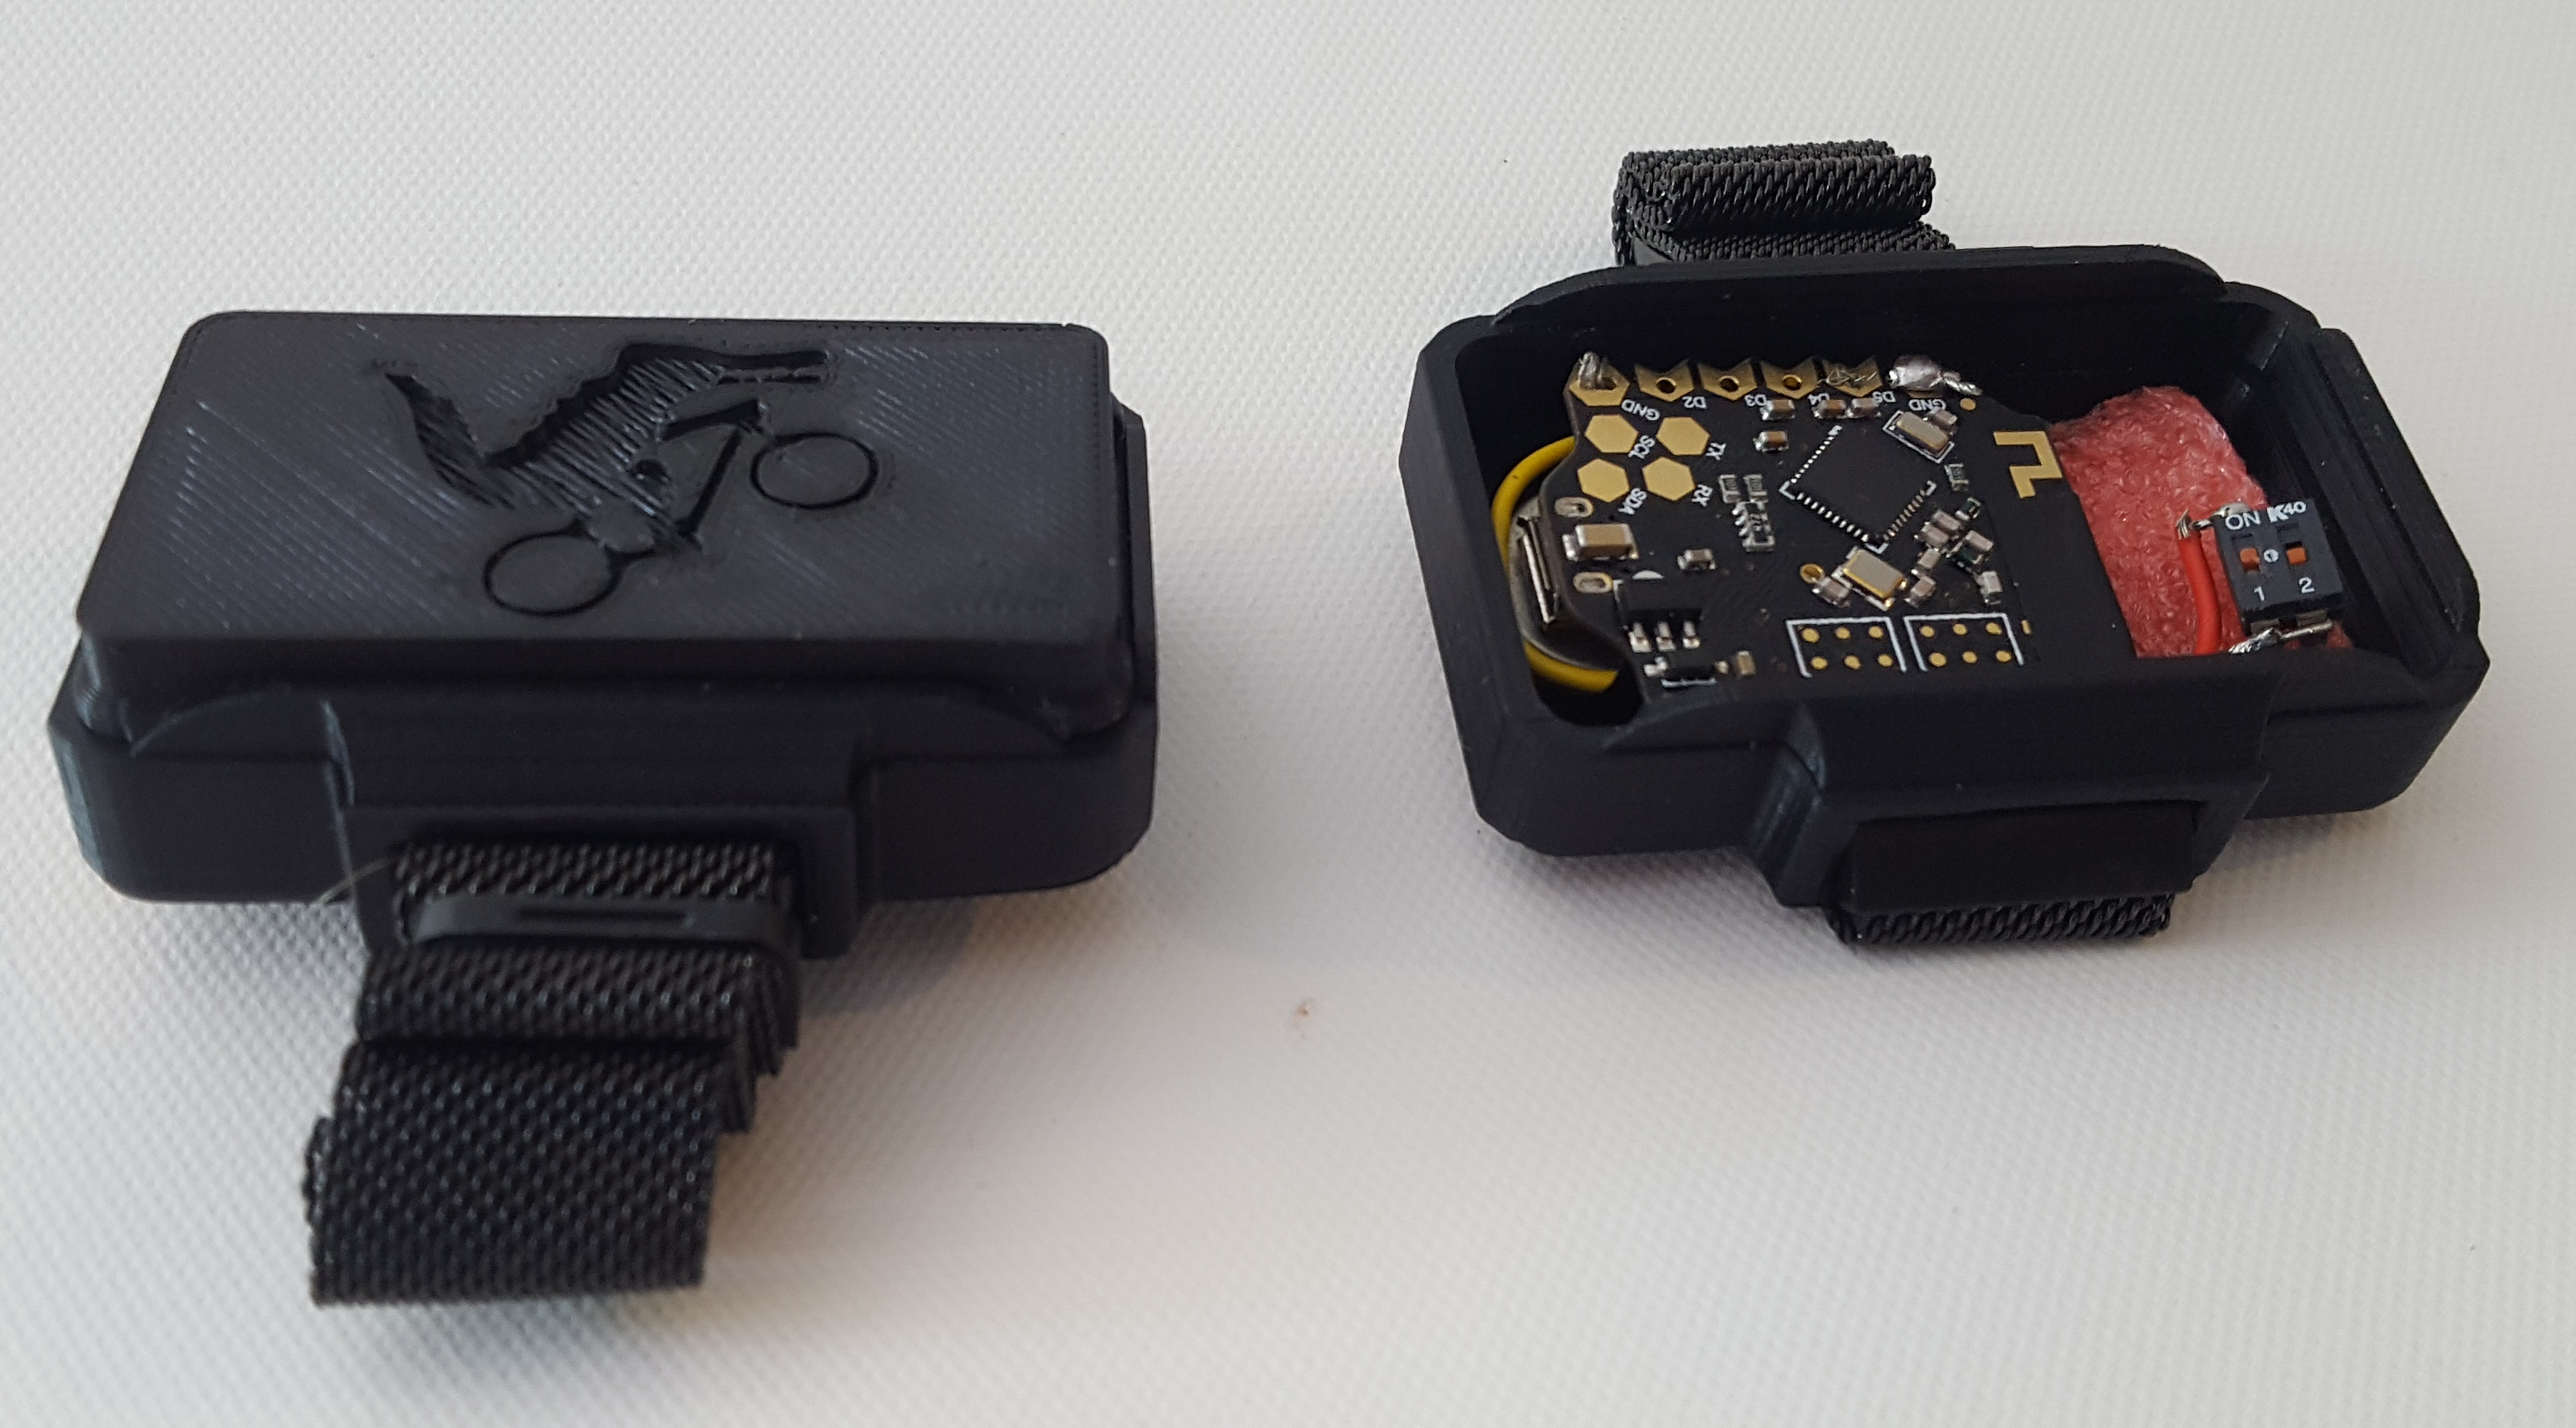
\includegraphics[width=1.02\columnwidth]{figures/product.png}
\caption{The developed wristbands with hardware. }\label{fig:product}
\end{figure}
A new Android application was also developed with a cleaner interface, ability to search addresses, more detailed route visualisation and a tutorial for the system. The Tutorial informs the user of the different instructions and demonstrates the different tactons.This lead us to a new lab test to examine how to design the different tactons for each instruction.

\section{Second Lab Test: Designing Tactons}
When designing different tactons for each navigational instruction it was determined to design four different tactons for each of five navigational instructions. The tactons were made based on two factors that can influence a tacton:\newline
Intensity - high and low 
Rhythm - slow and fast.
Based on these, four tactons were designed for each navigational instruction, where each tacton differentiated in intensity and rhythm. Intensity and rhythm were chosen to be the main factors because these are the parameters that influenced the distinguishability of tacton. 
\begin{table}
\centering
\small
\begin{tabular} {p{2.0cm}p{2.0cm}p{2.0cm}}
\toprule
 & \textbf{Low intensity} & \textbf{HIGH intensity}  
\tabularnewline 
\midrule
\textbf{Slow Rhythm} & Low/Slow & HIGH/Slow  
\vspace{0.1cm} \tabularnewline
\textbf{Fast Rhythm} & Low/Fast & HIGH/Fast 
\vspace{0.1cm} 
\tabularnewline
\bottomrule
\end{tabular}
\caption{The four way differentiation between tactons.}
\label{tab:stage_two_tacton_design}
\end{table}
\noindent
\newline
\newline
Each of the tactons were sent to the test participant three times, and afterwards the participant had to evaluate the tacton on the suitability based on the context of navigational instruction, and whether they liked it. This procedure was repeated till all 20 (four for each navigational instruction) tactons were evaluated.
\newline
\newline
This lab test showed that instructions that required immediate attention (Arrival, Problem), had to be HIGH/FAST or HIGH/SLOW, indicating that high intensity is important parameter when there is a need for attention. 
While navigational instructions that should stay in users periphery or inform users gradually (Heartbeat, U-turn and Turn) required low intensity and slow rhythm. This information was used when choosing the final tactons that were implemented in the system.  
\section{Second Field test}
The final field test was performed in the same settings as the first field test.The users were handed the system and had to themselves find out how to use it, with help from the tutorial in the mobile application. When they were familiar with the system - the test began. The same route was chosen as in the first field test with the same three destinations. 
\newline
\newline
The test participants were given one destination at a time and had to use the system to navigate to the location. After the field test, participants answered some interview questions, these were derived from the Calm Technology principles, this was done to evaluate the ''calm'' quality of the system. In total 19 people participated in the evaluation.
\begin{figure}[!b]
  \centering
  \includegraphics[width=1.02\columnwidth]{figures/stort_heat_map.png}
  \caption{The tracking of the 19 participants' routes for the field evaluation.}
  \label{fig:stort_heat_map}
\end{figure}
\subsection{Results}
In the evaluation it was found that the system performed well, and many test participants expressed that the system required less attention than traditional navigational systems, such as Google maps and GPS. 
\newline
\newline
Additionally, test participants trusted the system, even though some issues occurred during the navigation. The Heartbeat instruction was originally designed to assure the user that the system is functioning correctly. But the test proved the opposite, with participants explaining that the heartbeat was confusing and obtrusive to them. This was due to the fact that they were expecting instructions, and the heartbeat read to them as having to do some activity in response, when in actuality, it was only meant as assurance.
\newline
Another issues was with the turn instruction. The turn instruction works by starting at a waypoint when approaching a turn, based on speed and distance. When two turns was too close to each other, the tacton for the second turn would be started before the user had performed the first turn. This made them miss turns.
\newline
\newline 
However, even though they cycled in the wrong direction after missing a turn or due to other problems, no help was required from the test monitor to find the right way again, in contrary to the first field test.  Here the mobile application was usually used to see the route or to connect to the wearables again. 
\newline
Based on the interview, the majority of the calm technology principles were met in the system. 
\section{Conclusion}
Vibration worked well as an alternative way of sending navigational instructions. It was found to be unobtrusive, when only giving the relevant information, as required by Calm Technology principles. 
And even though it is important to inform and keep calm, the information should be considered carefully, since too much information can do the opposite of intended. This was the case in the second prototype, were heartbeat confused the participants. When designing tactons, it is important to make them clearly distinguishable, and it should be avoided to rely on the users ability to easily distinguish many different tactons. However it should be noted that some related work suggests that users can be trained to better distinguish tactons. 
\newline
The system is still too big for some test participants, and therefore developing an even smaller wearable would be optimal. 

\section{Acknowledgements}

% Balancing columns in a ref list is a bit of a pain because you
% either use a hack like flushend or balance, or manually insert
% a column break.  http://www.tex.ac.uk/cgi-bin/texfaq2html?label=balance
% multicols doesn't work because we're already in two-column mode,
% and flushend isn't awesome, so I choose balance.  See this
% for more info: http://cs.brown.edu/system/software/latex/doc/balance.pdf
%
% Note that in a perfect world balance wants to be in the first
% column of the last page.
%
% If balance doesn't work for you, you can remove that and
% hard-code a column break into the bbl file right before you
% submit:
%
% http://stackoverflow.com/questions/2149854/how-to-manually-equalize-columns-
% in-an-ieee-paper-if-using-bibtex
%
% Or, just remove \balance and give up on balancing the last page.
%
\balance{}

% REFERENCES FORMAT
% References must be the same font size as other body text.
\bibliographystyle{SIGCHI-Reference-Format}
\bibliography{sample}

\end{document}

%%% Local Variables:
%%% mode: latex
%%% TeX-master: t
%%% End:
